\documentclass{beamer}
\usepackage{pdfpages}
\usepackage{amssymb}
\usepackage{enumerate}
\usepackage{array}
\usepackage{lmodern}
\usepackage{url}
\usepackage{hyperref}
\usepackage[all]{xy}

%Farbschema
\definecolor{türkis}{rgb}{0.0, 0.65, 0.76}
\definecolor{weiss}{rgb}{1.0,1.0,1.0}
\definecolor{gruen}{rgb}{0.22, 0.74, 0.07}

\usetheme{metropolis}
%\usecolortheme{whale}
\setbeamercolor{progress bar}{fg=gruen,bg=gruen}
\setbeamercolor{frametitle}{bg = gruen}
\setbeamercolor{background canvas}{bg = weiss}
\setbeamercolor{footline}{fg=gray}
\setbeamerfont{page number in head/foot}{size=\scriptsize}
\setbeamercolor{title}{fg = black}
\setbeamertemplate{frame footer}{ \insertlogo{
\includegraphics[width=0.85cm]{img/aegis_logo_with_name.png}} \hfill  \insertsection}

%Information to be included in the title page:
\title[Abwehr von Denial-of-Service-Angriffen durch effiziente User-Space Paketverarbeitung: AEGIS]{Abwehr von Denial-of-Service-Angriffen durch effiziente User-Space Paketverarbeitung: AEGIS}
\subtitle{Review für die Planungs- und Entwurfsphase}
\institute{Technische Universität Ilmenau}
\date{27.05.2021}

\begin{document}

\frame{\titlepage}
\begin{frame}
    \frametitle{PROBLEMSTELLUNG}
    \begin{figure}[ht]
        \centering
        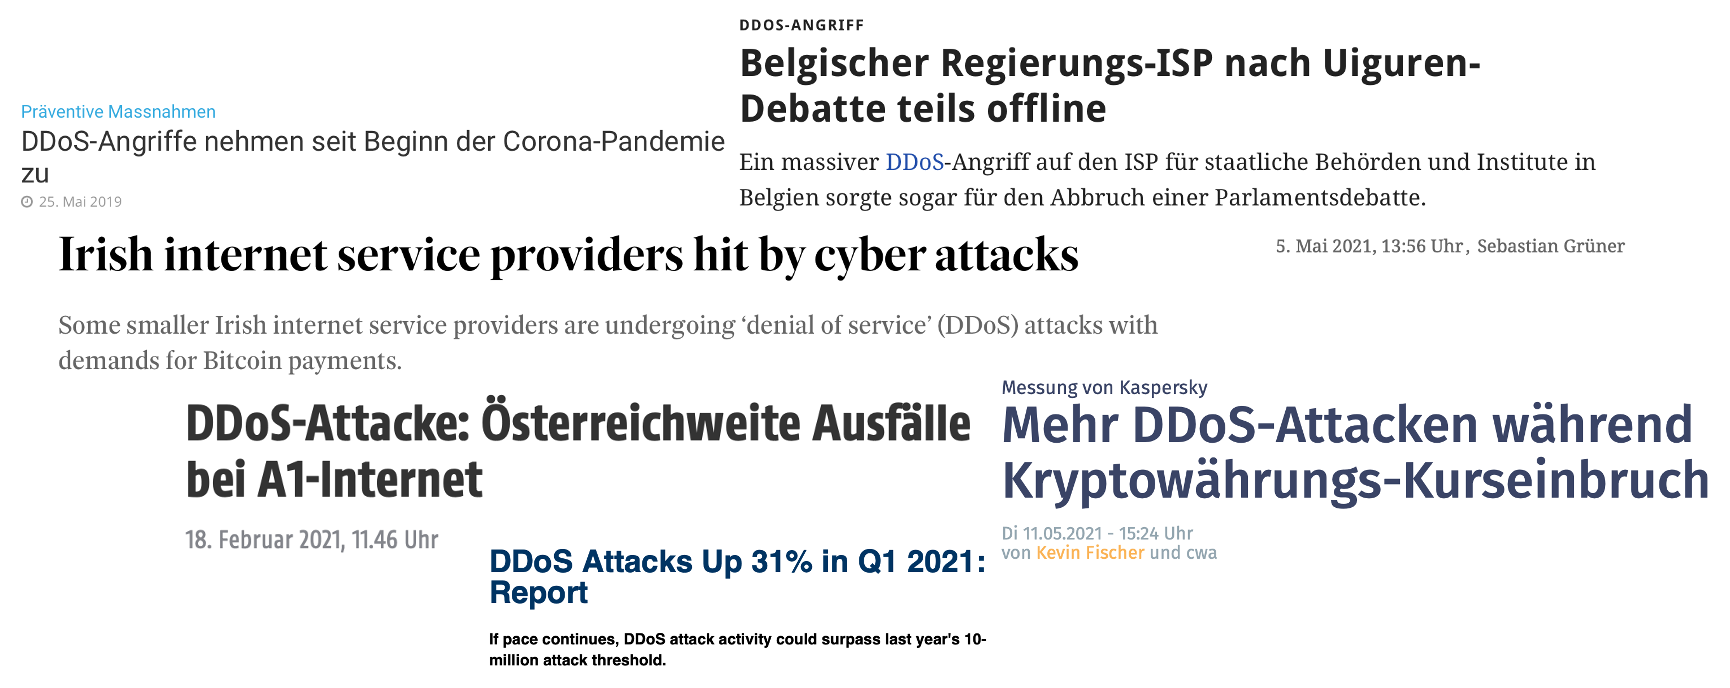
\includegraphics[width=11.5cm]{img/zeitung.png}
    \end{figure}
\end{frame}

%\begin{frame}
%    \frametitle{WAS SIND DOS-ANGRIFFE?}
%    \begin{figure}[ht]
%        \centering
%        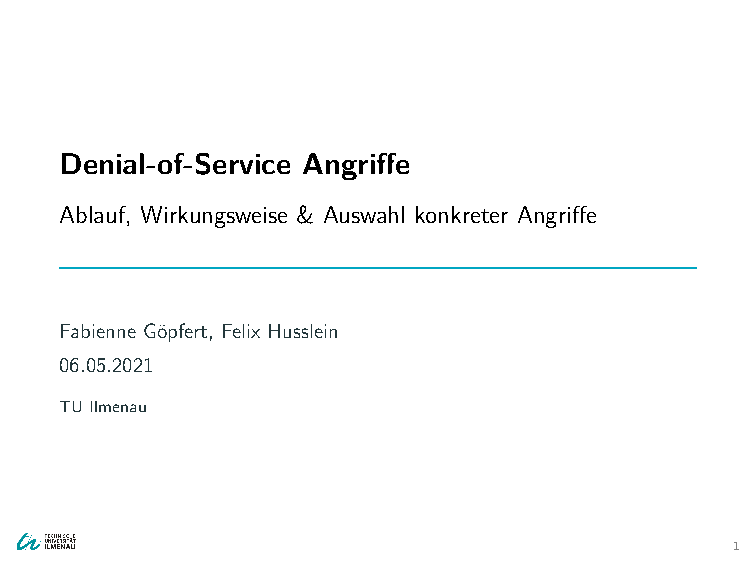
\includegraphics[width=8cm]{img/dos.pdf}
%    \end{figure}
%\end{frame}

\begin{frame}
    \frametitle{SYN-Flood}
    \begin{figure}[ht]
        \centering
        \includegraphics[width=10.5cm]{img/syn_flut_erklärung.png}
    \end{figure}
\end{frame}

\begin{frame}
    \frametitle{VORTEILE VON AEGIS}
    \begin{figure}[ht]
        \centering
        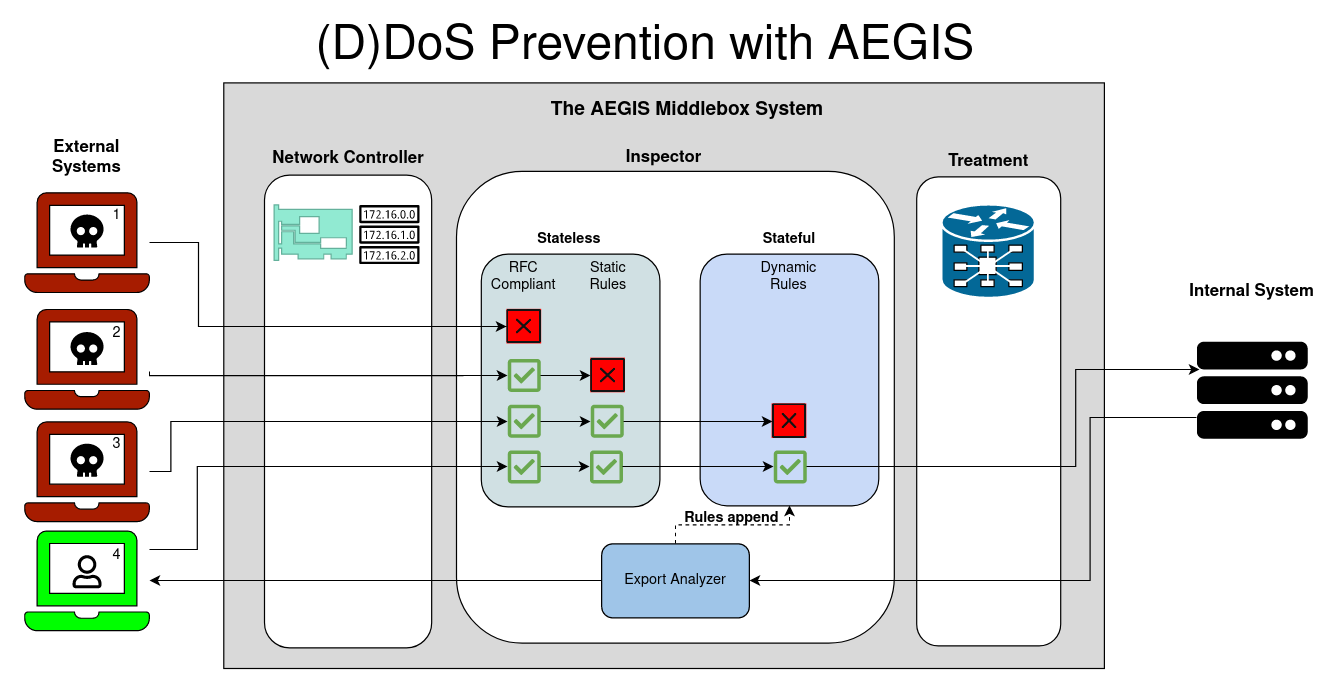
\includegraphics[height=5.5cm]{img/security_layers_vp_online.png}
    \end{figure}
    \vspace{-0.35cm}
    \begin{itemize}
        \item Paketverarbeitung im User-Space
        \item Nutzung effizienter Datenstrukturen
        \item Anvisierte Datenrate von 20-25 Gbit/s
    \end{itemize}
\end{frame}

%\begin{frame}
%    \frametitle{ANFORDERUNGEN}
%    \begin{figure}[ht]
%        \centering
%        \includegraphics[height=8cm]{img/anforderungen.pdf}
%    \end{figure}
%\end{frame}

%\section{Ergebnisse der Anforderungsanalyse}
\begin{frame}
    \frametitle{USE-CASE-DIAGRAMM}
    \begin{figure}[ht]
        \centering
        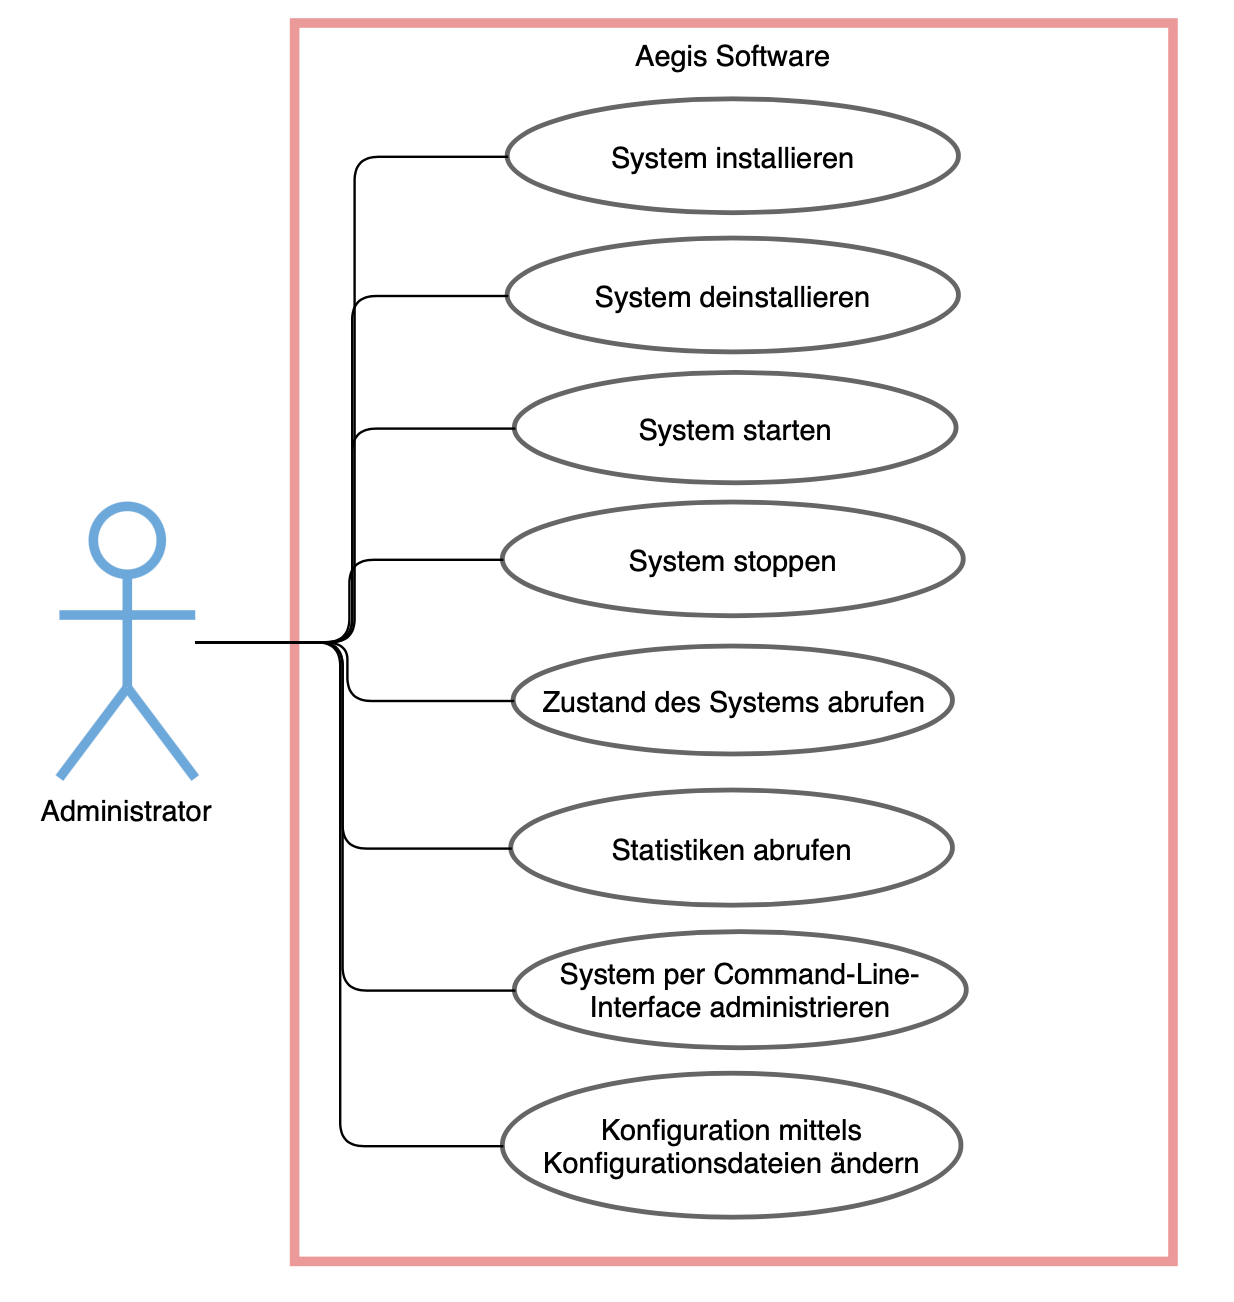
\includegraphics[height=8cm]{img/use_case_diagram_1.png}
    \end{figure}
\end{frame}

\begin{frame}
    \frametitle{PAKETDIAGRAMM}
    \begin{figure}[ht]
        \centering
        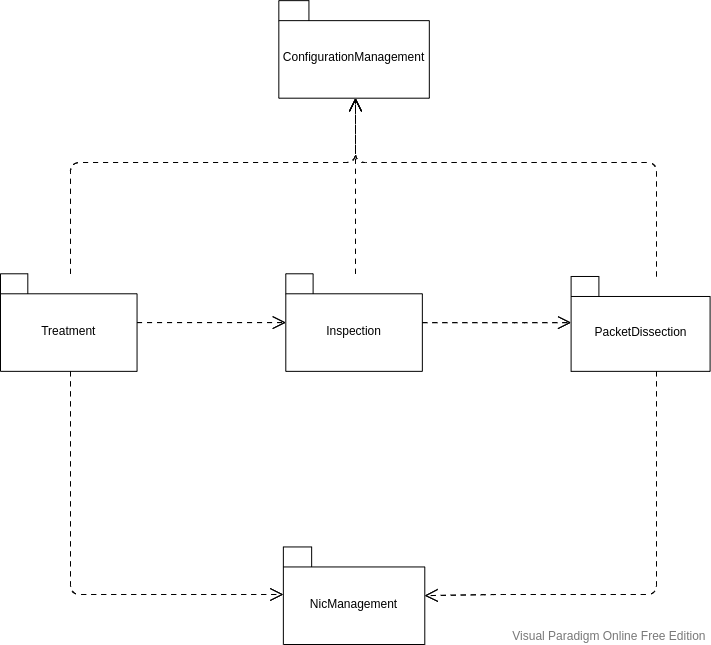
\includegraphics[height=7.5cm]{img/dos_paketdiagramm.png}
    \end{figure}
\end{frame}

%\begin{frame}
%    \frametitle{KLASSENDIAGRAMM}
%    \begin{figure}[ht]
%        \centering
%        \includegraphics[height=8cm]{img/class_diagram_new.pdf}
%    \end{figure}
%\end{frame}

\begin{frame}
    \frametitle{SEQUENZDIAGRAMM: SYN-FLOOD}
    \vspace{0.5cm}
    \begin{figure}[ht]
        \centering
        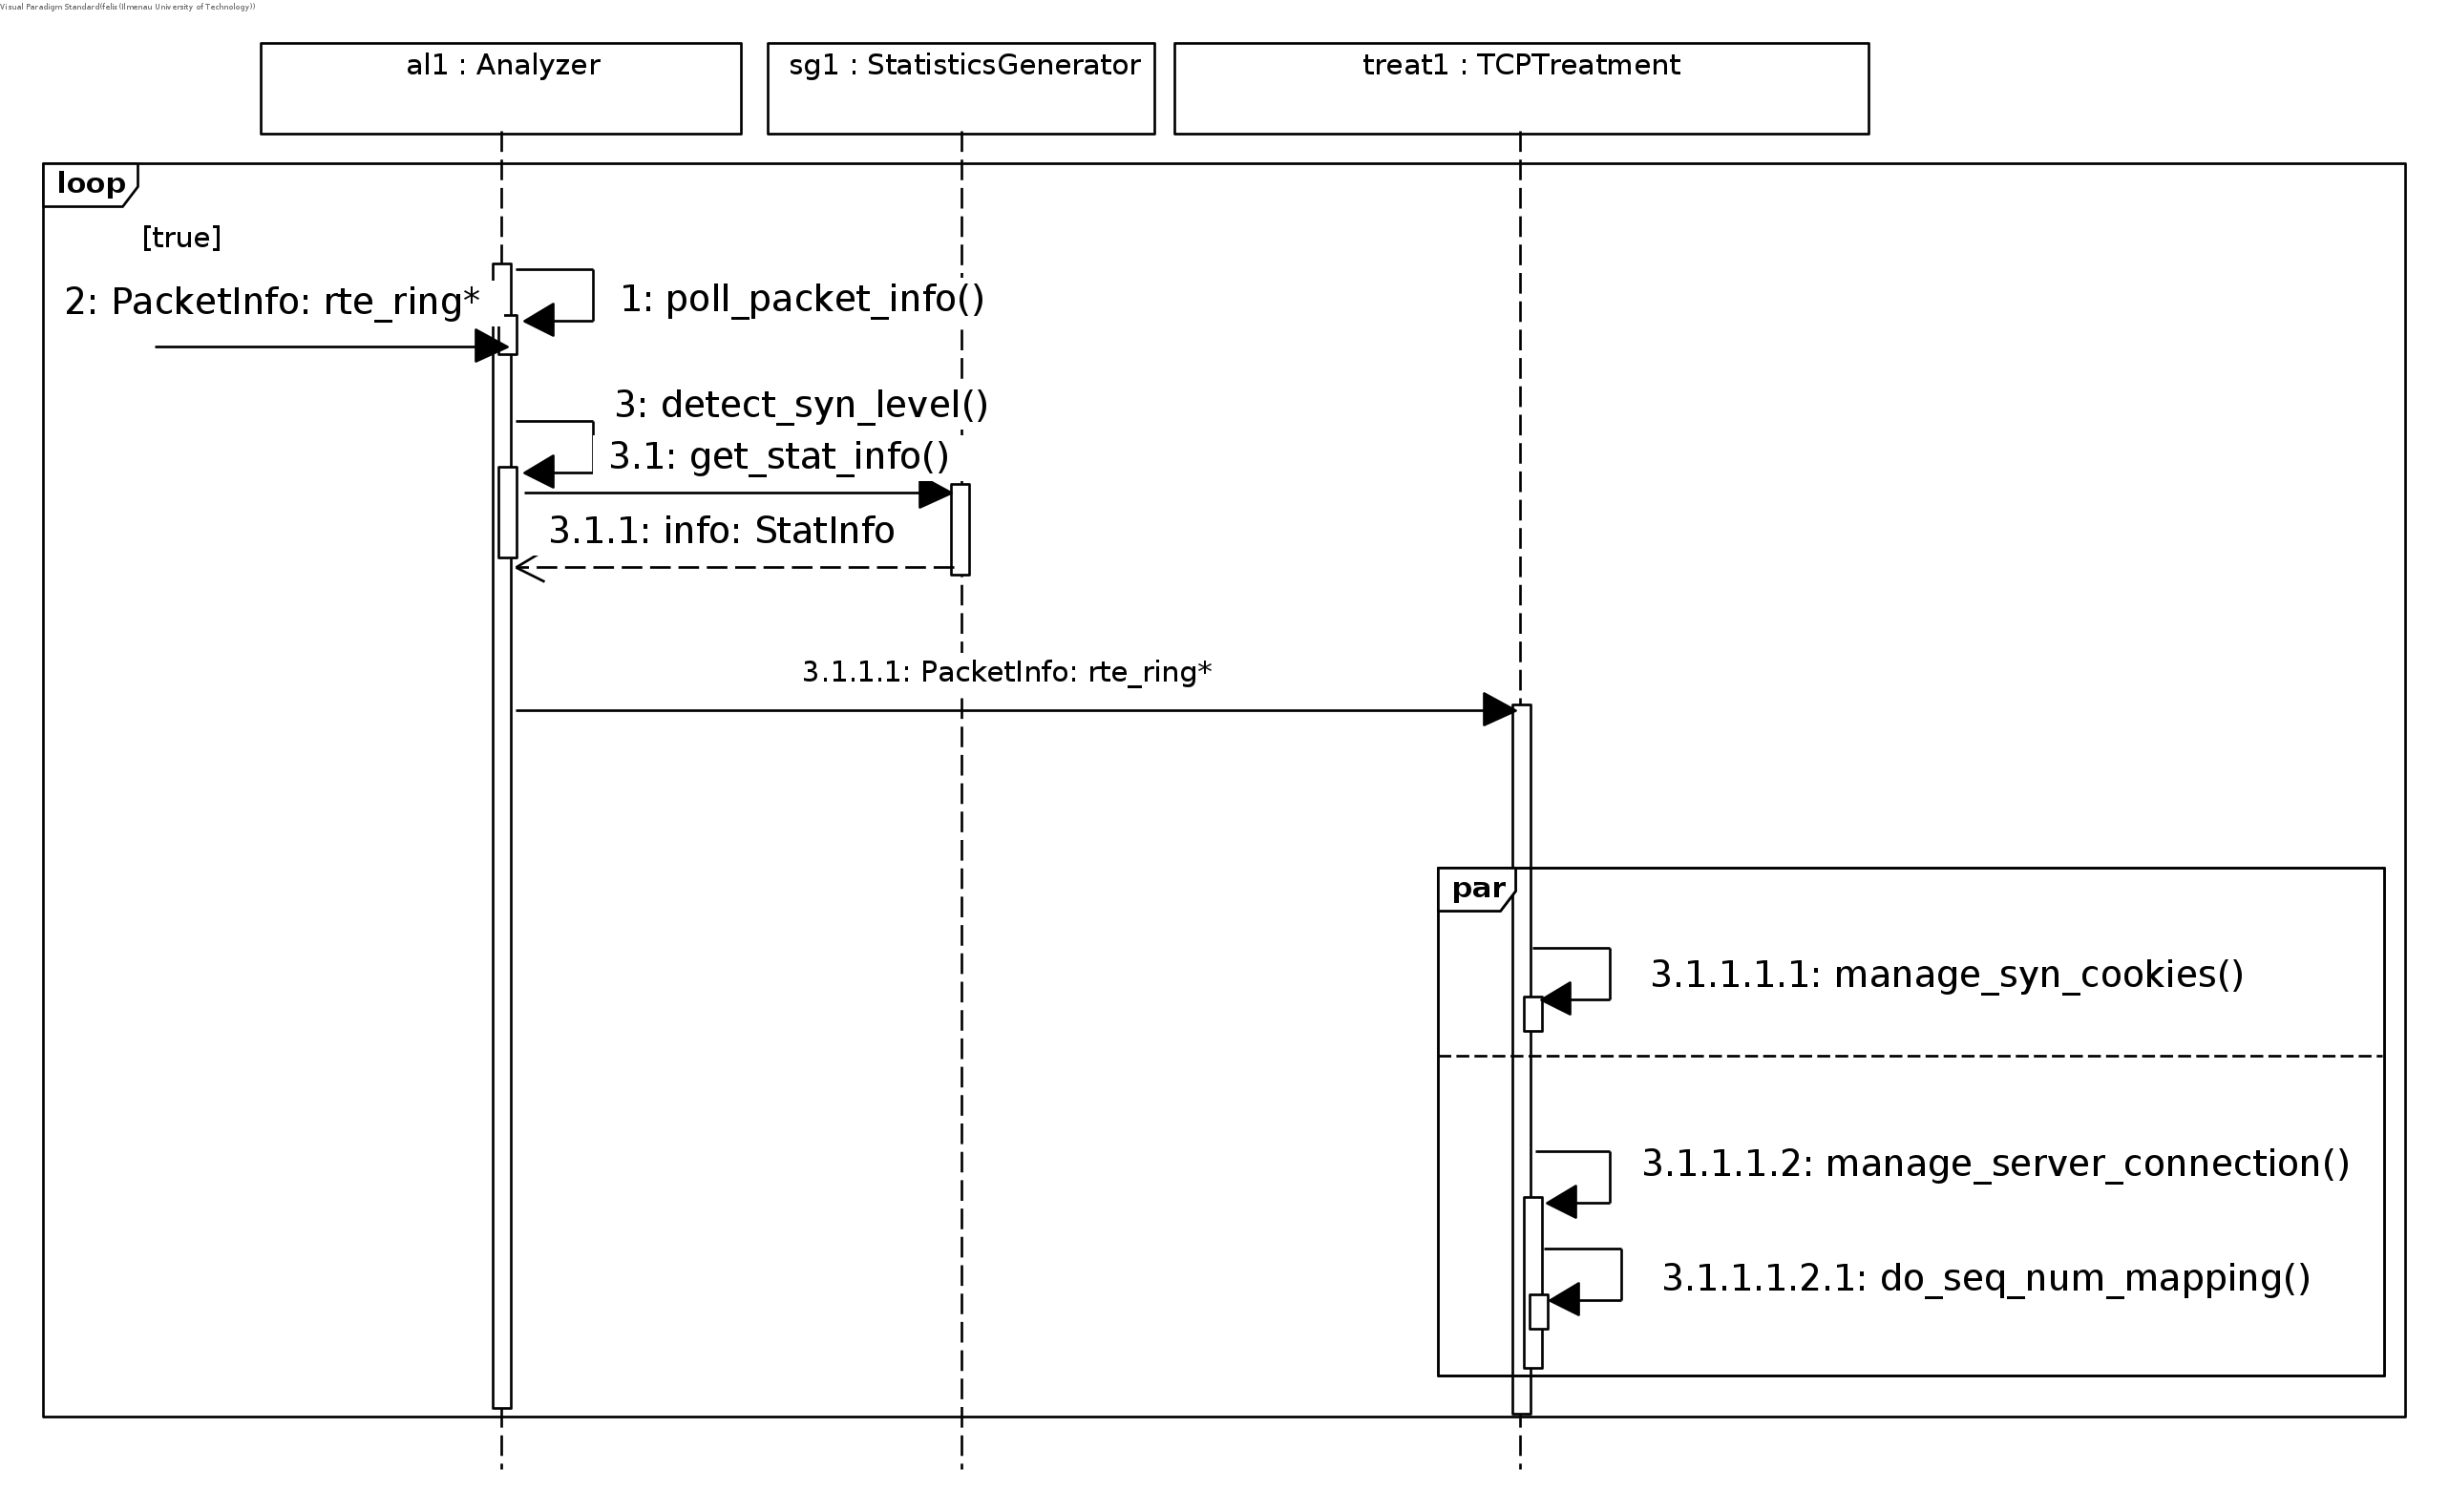
\includegraphics[height=6.5cm]{img/sequenzdiagramm_syn_flut.png}
    \end{figure}
\end{frame}

\begin{frame}
    \frametitle{TECHNOLOGIEN UND ENTWICKLUNGSWERKZEUGE}
    \begin{figure}[ht]
        \centering
        \includegraphics[height=6.5cm]{img/werkzeuge.png}
    \end{figure}
\end{frame}

%\begin{frame}
%    \frametitle{UNIFIED PROCESS +}
%    \begin{figure}[ht]
%        \centering
%        \includegraphics[width=11cm]{img/UnifiedProcess+.pdf}
%    \end{figure}
%\end{frame}

%\begin{frame}
%    \frametitle{GANTT-DIAGRAMM}
%    \begin{figure}[ht]
%        \centering
%        \includegraphics[width=11cm]{img/gantt.pdf}
%    \end{figure}
%\end{frame}

%\begin{frame}
%    \frametitle{AUFWANDS- UND RISIKOANALYSE}
%    \begin{itemize}
%        \item Aufwandsschätzverfahren COCOMO II: 2107h geschätzter Aufwand vs. 1800h nach den LP für das Softwareprojekt
%        \item Beispiel für ein ermitteltes Risiko (R02): Unzureichende Erfahrung des Projektteams bezüglich der Technologien
%    \end{itemize}
%    \begin{figure}[ht]
%        \centering
%        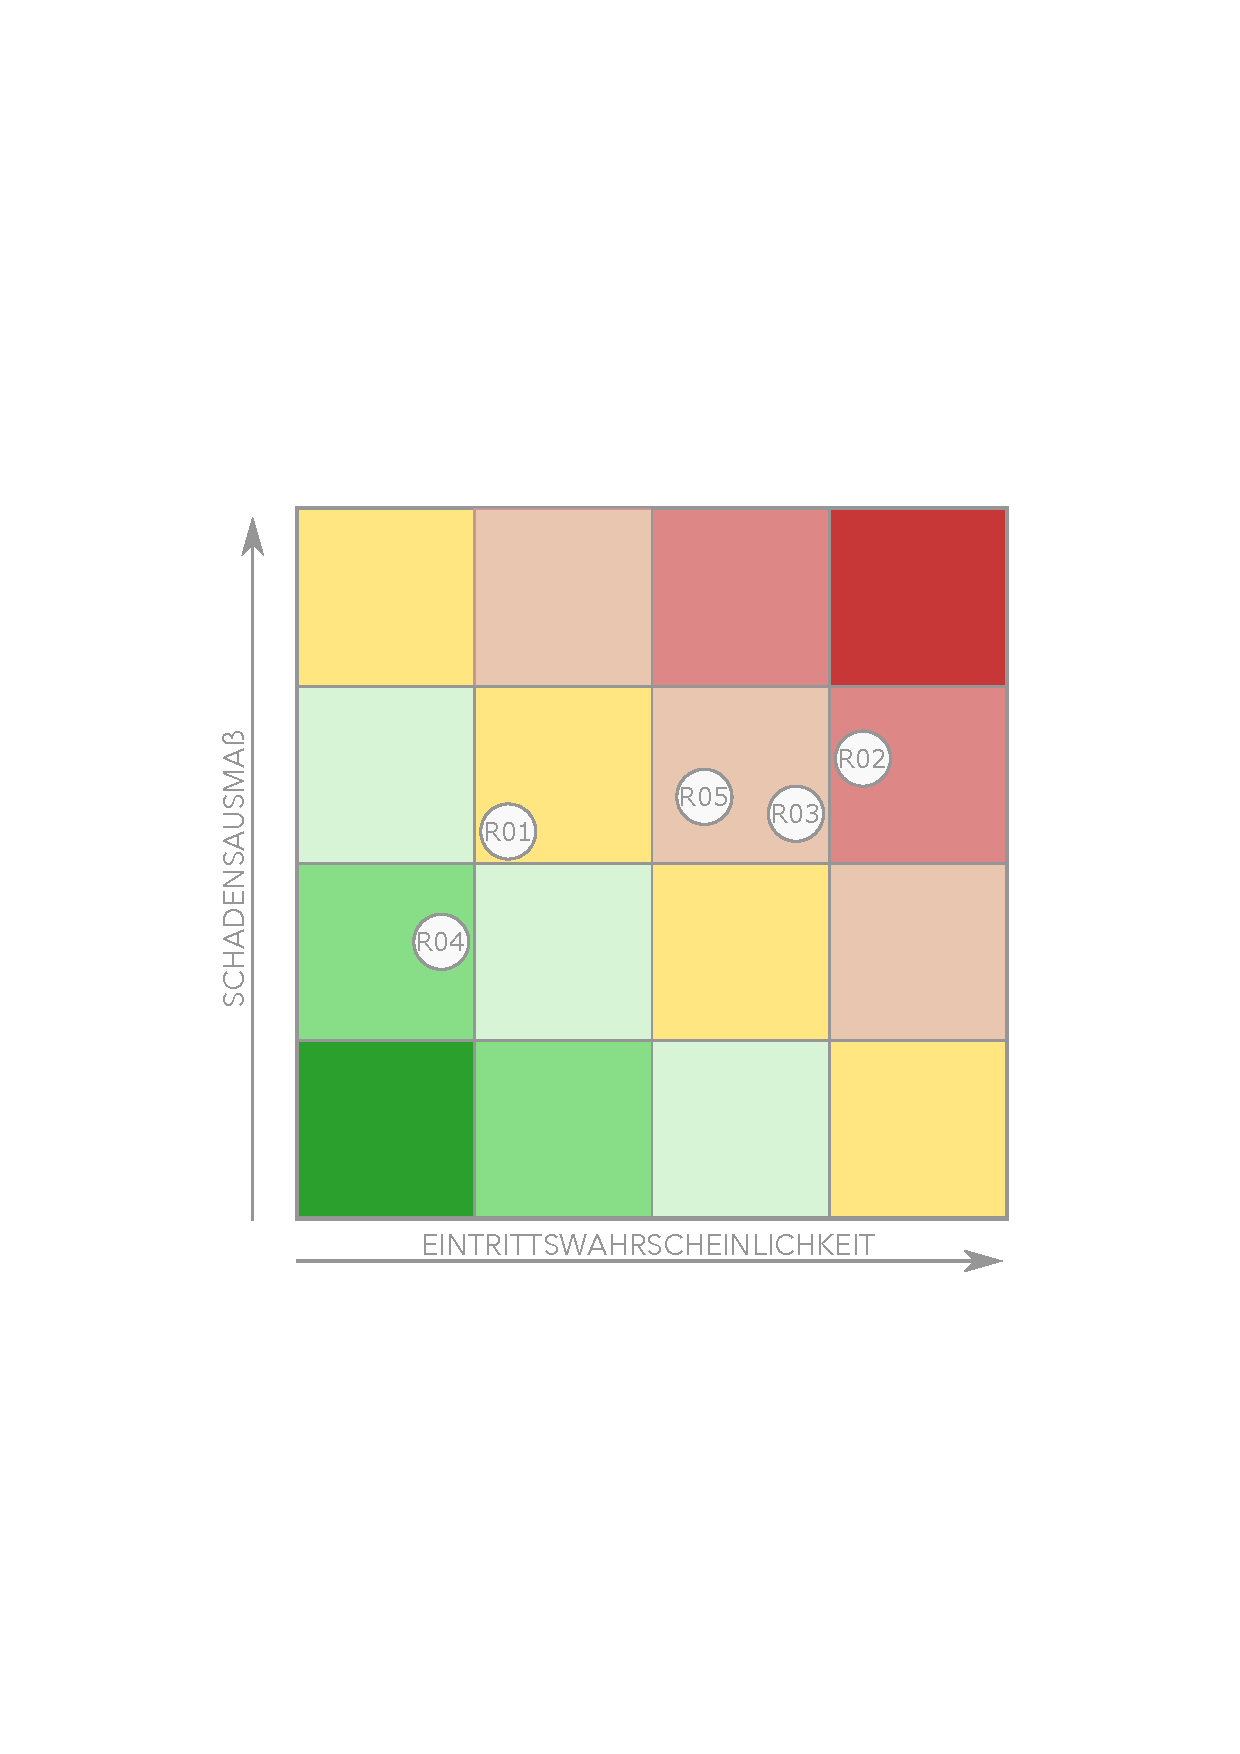
\includegraphics[height=5cm]{img/risikomatrix.pdf}
%    \end{figure}
%\end{frame}

\begin{frame}
    \frametitle{INTERNE ORGANISATION}
    \begin{figure}[ht]
        \centering
        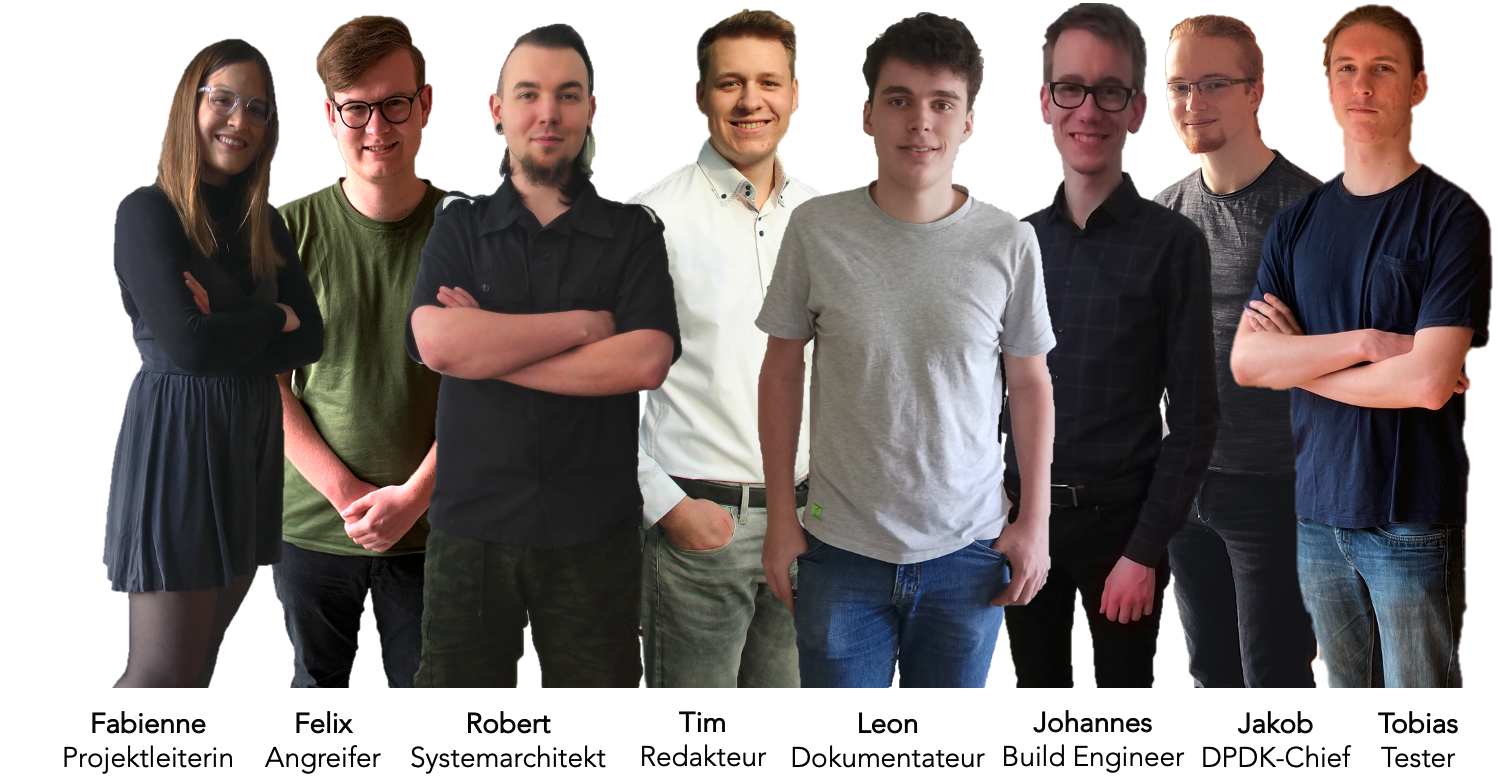
\includegraphics[width=11cm]{img/team_neu.png}
    \end{figure}
\end{frame}

\begin{frame}
    \frametitle{STAND DES PROJEKTS UND AUSBLICK}
    \begin{figure}[ht]
        \centering
        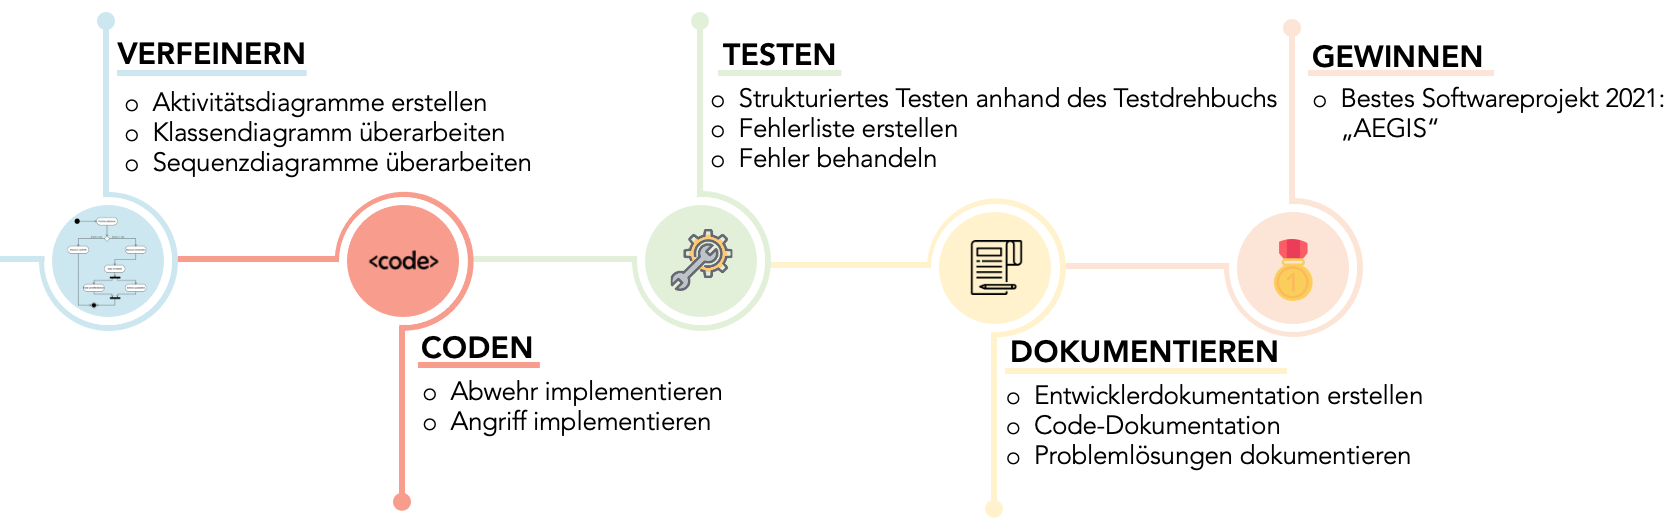
\includegraphics[width=11cm]{img/ausblick.png}
    \end{figure}
\end{frame}

\begin{frame}
    \frametitle{QUELLEN}
    \begin{itemize}
        \tiny
        \item Fischer, Kevin (11.05.2021): Messung von Kaspersky.
              Mehr DDoS-Attacken während Kryptowährungs-Kurseinbruch. Aufgerufen am: 24.05.21, von: \url{https://www.it-markt.ch/cybersecurity/2021-05-11/mehr-ddos-attacken-waehrend-kryptowaehrungs-kurseinbruch}
        \item Grüner, Sebastian (05.05.2021): DDoS-Angriff. Belgischer Regierungs-ISP nach Uiguren-Debatte teils offline.
              Ein massiver DDoS-Angriff auf den ISP für staatliche Behörden und Institute in Belgien sorgte sogar für den Abbruch einer Parlamentsdebatte. Aufgerufen am: 24.05.2021, von \url{https://www.golem.de/news/ddos-angriff-belgischer-regierungs-isp-nach-uiguren-debatte-teils-offline-2105-156275.html}
        \item DDoS Attacks Up 31\% in Q1 2021: Report. (17.05.2021). Aufgerufen am: 24.05.2021, von \url{https://www.darkreading.com/attacks-breaches/ddos-attacks-up-31--in-q1-2021-report/d/d-id/1341036}
        \item DDoS-Attacke: Österreichweite Ausfälle bei A1-Internet. (18.02.2021). Aufgerufen am: 24.05.2021, von \url{https://orf.at/stories/3201985/}
        \item Irish internet service providers hit by cyber attacks.
              Some smaller Irish internet service providers are undergoing ‘denial of service’ (DDoS) attacks with demands for Bitcoin payments. (18.05.2021) Aufgerufen am: 24.05.2021, von \url{https://www.independent.ie/business/technology/irish-internet-service-providers-hit-by-cyber-attacks-40441177.html}
        \item Zachow, Alexander(25.05.2019): Präventive Massnahmen.
              DDoS-Angriffe nehmen seit Beginn der Corona-Pandemie zu. Aufgerufen am: 24.05.2021, von \url{https://www.it-daily.net/it-sicherheit/cloud-security/28664-ddos-angriffe-nehmen-seit-beginn-der-corona-pandemie-zu}
    \end{itemize}
\end{frame}

\begin{frame}
    \begin{center}
        Vielen Dank für Ihre Aufmerksamkeit!
    \end{center}
\end{frame}

\begin{frame}
    \frametitle{NETZWERKPLAN}
    \begin{figure}[ht]
        \centering
        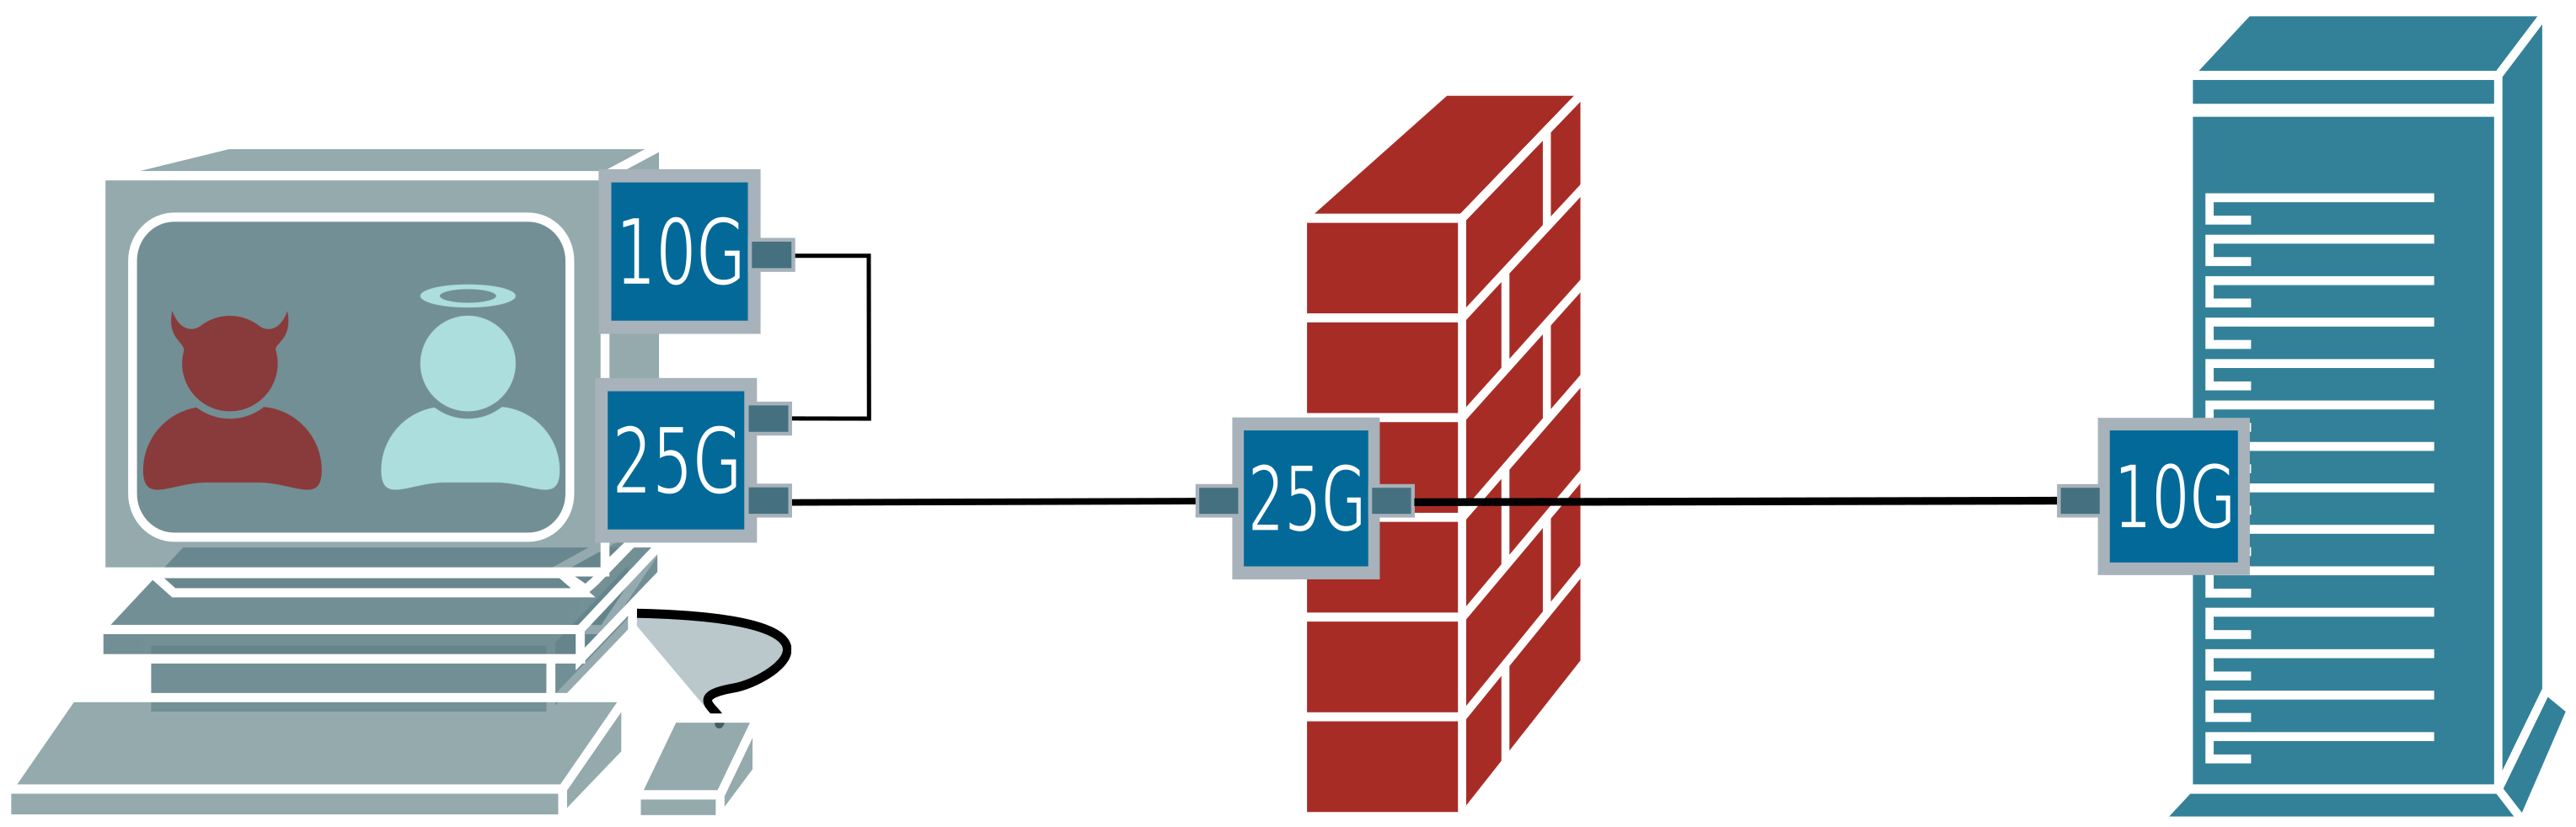
\includegraphics[width=11cm]{img/netzwerkplan.png}
    \end{figure}
\end{frame}

\end{document}
